% Source: graduate-coursework/Research/Papers/drafts/temporal_context_motion_trails/Radar_TemporalContext_MotionTrails.tex
% Description: Cross-location trend: optimal horizon varies with density and occlusion.

\documentclass[border=4pt]{standalone}
\usepackage{algpseudocode}
\usepackage{amsmath,amssymb}
\usepackage[T1]{fontenc}
\usepackage{pgfplots}
\usepackage{tikz}
\usepackage{xcolor}
\pgfplotsset{compat=1.18}
\usetikzlibrary{arrows.meta,positioning,calc,fit,shapes.geometric,shapes.misc,decorations.pathmorphing,backgrounds}


\newcommand{\ph}[1]{\textcolor{red}{#1}}

\begin{document}
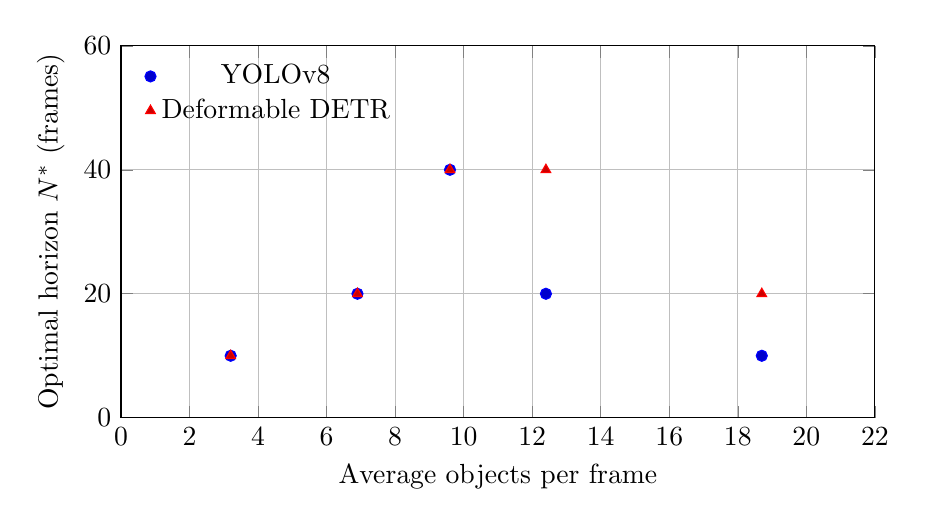
\begin{tikzpicture}
\begin{axis}[
  width=0.92\linewidth,
  height=0.52\linewidth,
  xlabel={Average objects per frame},
  ylabel={Optimal horizon $N^*$ (frames)},
  xmin=0, xmax=22,
  ymin=0, ymax=60,
  grid=both,
  legend style={at={(0.02,0.98)},anchor=north west,draw=none,fill=none},
]
\addplot+[only marks, mark=*] coordinates {(3.2,10) (6.9,20) (12.4,20) (18.7,10) (9.6,40)};
\addlegendentry{YOLOv8}
\addplot+[only marks, mark=triangle*] coordinates {(3.2,10) (6.9,20) (12.4,40) (18.7,20) (9.6,40)};
\addlegendentry{Deformable DETR}
\end{axis}
\end{tikzpicture}
\end{document}
